% Implementation
\chapter{Submodule implementations}

In order to test the viability and usefulness of Rust in the field of game engine development, the author implemented three common submodules of an engine. Because measurements of the Rust implementations alone would not be enough to tell how well or badly Rust performs in certain disciplines, all modules were also implemented in C++, serves as a baseline of the Rust module benchmarks. The systems that were selected for implementation were based on their importance and impact onto the performance of an engine and its tool suite. The first module that was implemented is a memory management system featuring rather low-level custom allocators, debugging facilities and an abstraction type that allows for combining them for more ergonomic and flexible use. The second one includes three different types of containers usable by an engine or its tools, showing how Rust handles mid-level systems, shared across an engine's core system and tool applications. The last module that was implemented features an \ac{ECS}, testing Rust's capabilities and ergonomics in a high-level system. 

This chapter is going to describe the general architectural overview of the research engine called \textit{Spark} \footnote{Name is based on the fact that it can either turn into a wildfire spreading if Rust's performance meets expectations or stop burning if it shows that it is not a competitor of C++ in any field.}. It will also shortly give an insight into the development environment of the C++ and Rust projects and is then followed by detailed descriptions of the systems \acp{API}. This will include both, general implementation details shared among the languages and differences between them. Basic code samples showcasing use cases of the systems will highlight advantages of the implementations and pitfalls that can occur when being used wrong.

\section{Spark engine architecture}

Following the concept of separated modules the current design implements each system as a standalone library. The basis of all three modules is built by a collection of common functionality grouped inside the \textit{core} library. It includes mostly functions often used in all modules. On top of the \textit{core} library, the other three engine systems are built, every single one being a standalone library without any dependencies to their siblings. This lack of dependency grants the benefit of being able to use every single one of these modules on their own. This concept is useful in the thesis's context to ensure that every system can be measured on it's own, without suffering any penalty when a depending module was implemented in a non optimal way. In a real world example the container system may be dependent upon the memory management to allow a programmer to choose the allocators used for a collection. And then again the \ac{ECS}, because it is more high-level and therefore it is allowed to depend onto lower level modules, could be built on top of the container library to use already implemented collections for holding components. But due to the need for independent measurements the author decided to follow the architecture that can be seen in Figure \ref{fig:spark_arch}.

\begin{figure}[h!]
	\centering 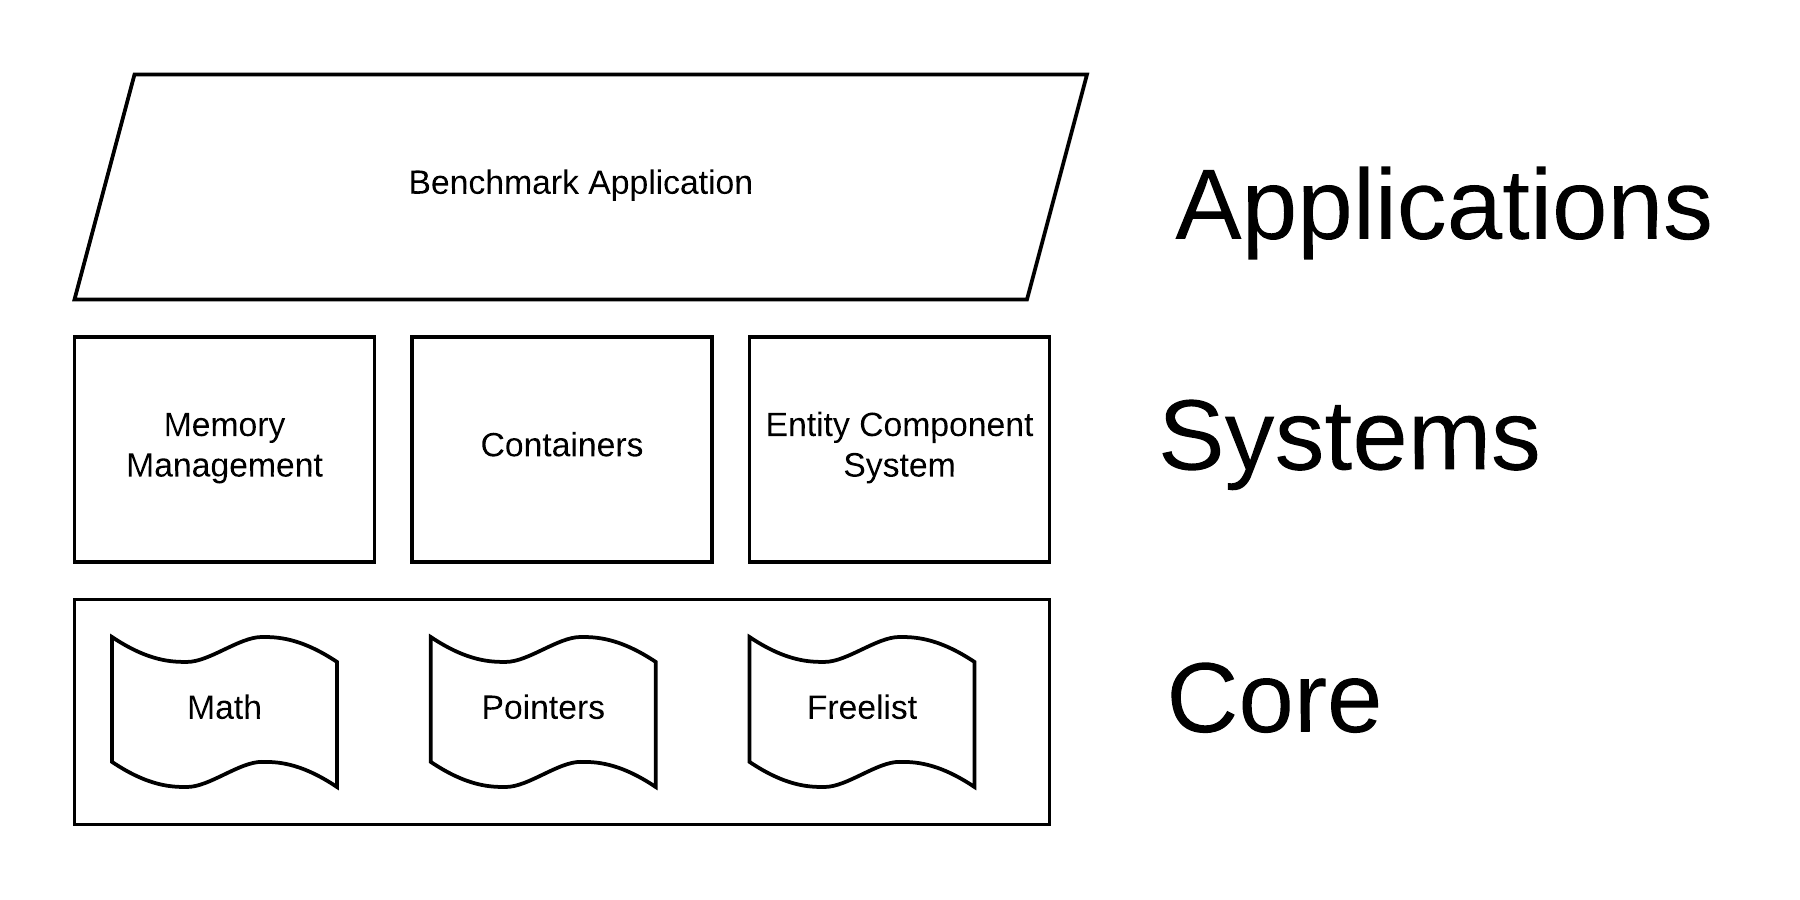
\includegraphics[width=\linewidth]{PICs/spark_arch.png}
	\caption{Layers of the module architecture implemented during this thesis. Higher layer can depend onto lower ones.}
	\label{fig:spark_arch}
\end{figure}

As it can be seen in the illustration above, the application used for benchmarking the different modules is built on top of them. This architecture is the same for both projects. Beside the shown components every project also contains a test suite, containing unit-tests for the features of all systems. How the tests are written and why the author decided to implement them additionally to the systems is described in the next section.

\section{Development process}

After the global architecture of the implementation was described this sections gives an insight into the development process of it. During the whole implementation period the author followed a test-driven approach for implementing features. Without going into much detail right now, it can be said that for every feature created there were several test cases developed beforehand describing the preferred usage and expected behavior of the \ac{API}. Exact details of this are described in section \ref{tdd}, which also describes what frameworks were used and what benefit can be gained by implementing tests. Because Rust is rather young and so is the \ac{IDE} world around it, the first part of this section will shortly explain which tools were used and how they compare to the ones used in C++, a mature language with a well-grown tooling landscape.

\subsubsection{Spark++ - the C++ project}

With Windows as the development \ac{OS} the straight forward \ac{IDE} choice for the C++ project was Visual Studio 2017. Because it is planned to develop the systems for multiple platforms in the future, \textit{premake} was used to create \ac{IDE} projects for the different platforms. \textit{Premake} is a build configuration system used for generating project files for Visual Studio, XCode or other \acp{IDE}. When creating configuration files with premake, one uses \textit{Lua}, a well-known scripting language in the gaming industry. An excerpt of the build configuration used for the C++ project can be seen in Listing \ref{lst:premake5_conf}.\\

\begin{lstlisting}[caption={Part of the premake.lua file used to generate the Spark C++ project files}, label={lst:premake5_conf}, language={[5.0]Lua}]
project "MemorySystem"
kind "StaticLib"
language "C++"
targetname "mem-sys"
targetdir "build/mem_sys/%{cfg.buildcfg}"

files { "src/MemorySystem/**.h", "src/MemorySystem/**.cpp" }

links { "Core" }
includedirs { "src/Core/"}

filter "configurations:Debug"
symbols "On"
flags { "StaticRuntime" }

filter "configurations:Release"
symbols "Off"
flags { "StaticRuntime" }
\end{lstlisting}

\noindent
The above script shows how the project for the memory system is setup. The description defines what kind of binary out shall be created and the most common one can be an executable, a static or dynamic library. A project description also contains binary dependencies and needed include files, as well as a location for all files that are part of the generated project. By using filter it is also possible to define certain settings that only take effect in specific build configurations. In the context of this thesis premake was only used to generate the Visual Studio solution but simplifies the process of porting the systems to other platforms. While \textit{premake} was only used for the C++ part of the implementation, the Rust one is based upon \textit{Cargo} and its setup is described in the next section.

\subsubsection{RustySpark - the Rust project}

Before the author settled for Visual Studio Code as the \ac{IDE} for Rust, there was an attempt on using Visual Studio too. But after a view hours of trying to work with the Rust plugin for it, developed by parts of the Piston engine community, the author decided to switch to \textit{VS Code}. That decision was based upon experiences of other Rust users and due to the author's experience with the Rust plugin. When using \textit{VS Code} a programmer benefits from useful extensions for Rust development and the usage of a tool called \textit{Racer}. Racer can be found at \url{https://github.com/racer-rust/racer} and is a utility for Rust code completion, boosting productivity and helps Rust newcomers. The build process was then totally done via \textit{Cargo's} exposed functionality. 

\subsubsection{Test-driven development} \label{tdd}

Another important part of the development process, apart tooling that supports the programmer, was the decision to follow a test-driven approach. The term \textit{test-driven development} in the context of the subsystem implementation describes the process of defining the wanted behavior in test cases and then implement functionality to pass these tests. For every feature several unit-tests were implemented to ensure that the behavior of small, separated parts of the software meet expectations. Beside the benefit of a structured development process another advantage of a well-maintained test-suite is the possibility to catch regressions introduced when altering or refactoring code. This safe-guard proved useful more than once during the development process and ensured that the behavior did not change when refactoring code or moving reusable functionality into the core library. The tests for the C++ project were implemented using the \textit{Google Test Framework} that proved to be quite easy to integrate while providing direct integration into Visual Studio. The tests of the Rust project where implemented directly in the different module files and were executed via the \texttt{cargo test} command. The fact that Rust projects come with an unit-test runner out-of-the-box is a great benefit for productivity and maintainability of code. 

\section{Memory Management} \label{mem_impl}

The first implemented submodule that is going to be described is the memory management system. As it was already mentioned in section \ref{mem_theory}, an engine's memory management system is responsible to provide control over how resources are used at runtime. It tries to reach peek performance by assuming access patterns and providing different allocation strategies. Beside that is important to provide debugging facilities, especially when working with pointers and raw memory. This section will first describe the general \ac{API} and from which parts the module is composed of. It will then highlight some interesting implementation details of both languages with code samples.

The design decisions for parts of the memory system are based on resources hosted at \textit{Stefan Reinalter's} blog \textit{Molecular Musings} \cite{MOL_MS_1} \cite{MOL_MS_2} \cite{MOL_MS_3} \cite{MOL_MS_4} \cite{MOL_MS_5} and on allocation strategies described in the book \textit{Game Engine Architectures} \cite{GEA_2}. The implementation for both languages share a common \ac{API} and at least the same system members. On top of that the Rust implementation features an additional abstraction layer to showcase how a safe interface for unsafe code can be built in Rust. The system is structured into the following parts:

\begin{labeling}{bounds checker}
	\item [allocator] facility to allocate and deallocate memory - providing different kinds of allocation policies
	\item [bounds checker] debugging facility to ensure the validity of an allocated memory area
	\item [memory realm] a memory allocation facilty that combines different 
	debugging facilities with allocation policies - flexible and policy-based approach
\end{labeling}

\subsection{Virtual memory}
\blindtext

\subsection{Allocators}

The different allocation strategies implemented serve as the module's basis. In order to allow a user to store them in a polymorphic way, all of them share a common interface. This interface is implemented as a pure virtual class in C++ and as a trait in Rust. The \ac{API} all of them share is shown in Listing \ref{lst:mem_api}. Although it showcases the C++ methods, the Rust trait only differs syntactically.\\

\begin{lstlisting}[caption={Common interface among all allocator implementation. Rust trait only differs syntactically from this C++ sample.}, label={lst:mem_api}, language={C++}]
class AllocatorBase
{
public:
virtual void* Alloc(size_t size, size_t alignment, size_t offset) = 0;
virtual void Dealloc(void* memory) = 0;
virtual void Reset() = 0;
virtual size_t GetAllocationSize(void* memory) = 0;
virtual ~AllocatorBase() = 0;
};
\end{lstlisting}

\noindent
Every allocator can fulfill an allocation request, that provides size, alignment and an optional offset of the allocation.  The term \textit{alignment} is related to an address a certain object resides at in memory. A certain value is said to be aligned to X, where X is a power of two and the address is a multiple of X. Normally alignment is not a concern to the everyday programmer but in certain situations and on specific hardware explicit alignment of values can yield better performance. The offset parameter describes how much memory the allocator shall provide \textbf{before} the aligned pointer. This is an important capability when an allocator is combined with a debugging facility that needs to store meta information in front of the aligned user pointer. 

The first allocation policy, that is also the most simple one, is a \textit{linear allocator}. It provides allocations with nearly zero overhead by not allowing the deallocation of single memory blocks. When using a linear allocator, the only possibility to free allocated blocks is to reset the whole buffer. Because of this fact it is not necessary to store the order of allocations and additional meta data needed when the internal pointer has to be rearranged on deallocations. Whenever an allocation is issue to the linear allocator, internally it ensures alignment and offset requirements and then bumps a pointer, pointing to the next free space. The only meta information that needs to be stored by the allocator is a 32-bit unsigned integer, storing the allocation's size. This is needed to properly work when used in the memory realm, which is described later. Figure \ref{fig:linear_alloc} visualizes the change in a linear allocator's internal state after an allocation request was issued.

\begin{figure}[h!]
	\centering 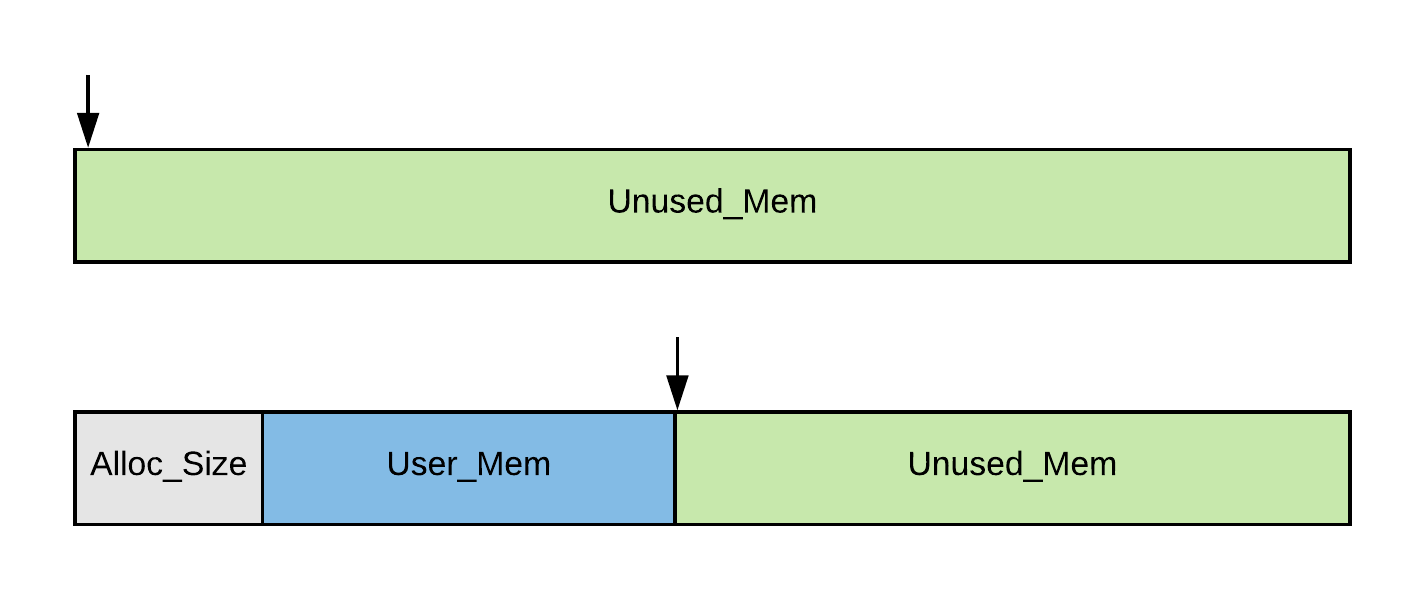
\includegraphics[width=\linewidth]{PICs/linear_alloc.png}
	\caption{A linear allocator's internal state before and after an allocation request.}
	\label{fig:linear_alloc}
\end{figure}

\noindent
A common use case for such an allocation strategy is allocating per-frame temporary values that can be freed all at once with the start of the next frame. 

If there is the need to free individual allocations another low overhead allocator can be used. A \textit{stack-based allocator} issues allocation requests by advancing the internal pointer forward, but it also provides the possibility to free single allocations again. One constraint though, assuming the usage pattern for better performance, is the order in which allocations can be freed. A stack-based allocator only allows deallocations to happen in the reverse order of the allocations, meaning it adheres to a \ac{LIFO} approach. In order to set the internal pointer back to a previously done allocation, the meta data size grows and so the overhead for any allocation is slightly larger than with a linear allocator. Figure \ref{fig:stack_alloc} shows the internal state of a stack-based allocator and how it is changed after an allocation and a deallocation.

\begin{figure}[h!]
	\centering 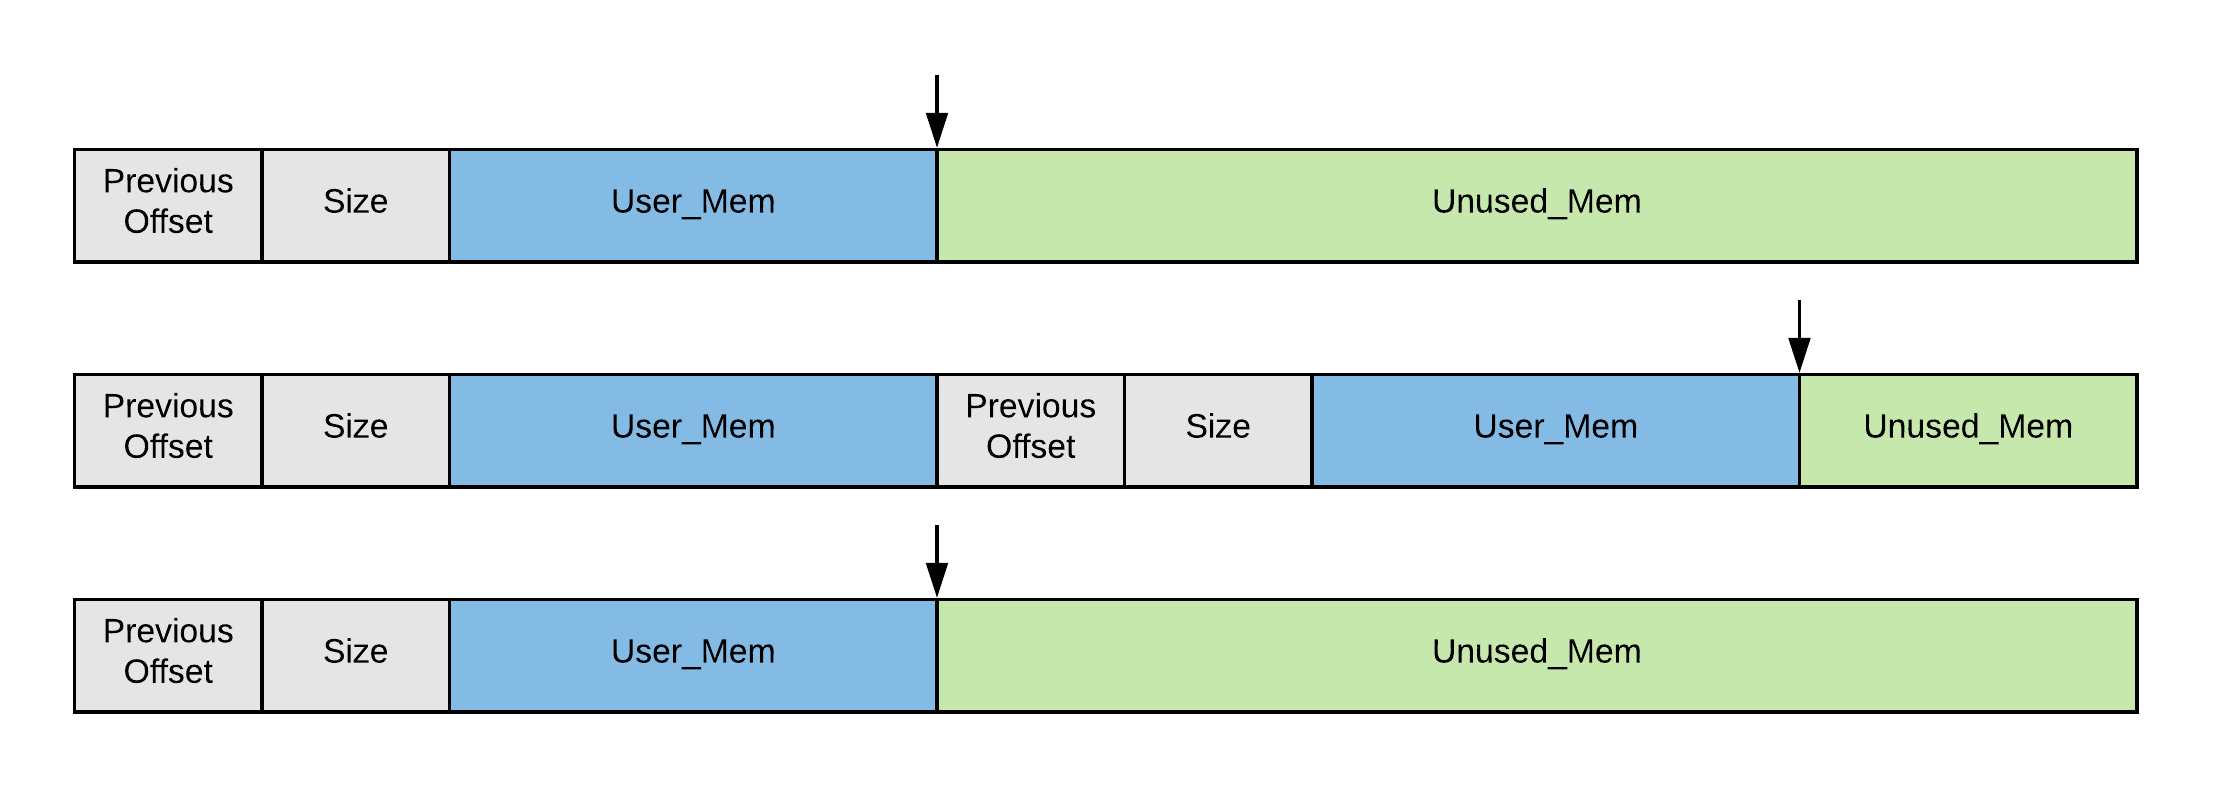
\includegraphics[width=\linewidth]{PICs/stack_alloc.png}
	\caption{A stack-based allocator's internal state before and after an allocation request, followed by a deallocation of a single block.}
	\label{fig:stack_alloc}
\end{figure}

\noindent
Compared to Figure \ref{fig:linear_alloc} it can be seen that the meta information in front of a user's memory block, from now on called the \textit{allocation header}, has grown. Additionally to the memory block's size it also stores an offset to the allocator's beginning, again using an 32-bit unsigned integer for it. The allocation header now introduces an overhead of 8 byte. But with this initial bit of information the internal pointer can be reset to its location before the last allocation. It is also exactly that behavior which forbids deallocation in any other order than the \ac{LIFO} one. If a block not coming from the last allocation would be freed, the allocator would create a hole and corrupt the internal pointer, preventing all other currently allocated blocks from being freed. The allocator's implementation features a second mode that runs a \ac{LIFO} check on every allocation at the cost of an additional 4 bytes overhead. If the mode is activated by using conditional compilation flags, these 4 bytes are used to store an allocation id. On every deallocation the stored id has to match the allocator wide counter or else the \ac{LIFO} rule was not respected. Common usage examples for this kind of allocation strategy include level loading, where certain values can be rolled back in reverse order after a level has finished.

An extension that can be built upon a stack-based strategy is the one of a \textit{double-ended stack allocator}. The process of allocating memory does not change compared to the underlying stack policy. But the novel feature of this approach is that the allocator can grow from both sides. Memory can be requested from either the front- or the back-end, allowing for better utilization of the allocator's space. While the per-allocation overhead does not grow, one additional pointer has to be stored in the allocator to track the current state of the back-end. Figure \ref{fig:double_stack_alloc} visualizes how such an allocator can grow and shrink from both sides and an interested reader can already guess what possible problems can occur and needs additional checks. 

\begin{figure}[h!]
	\centering 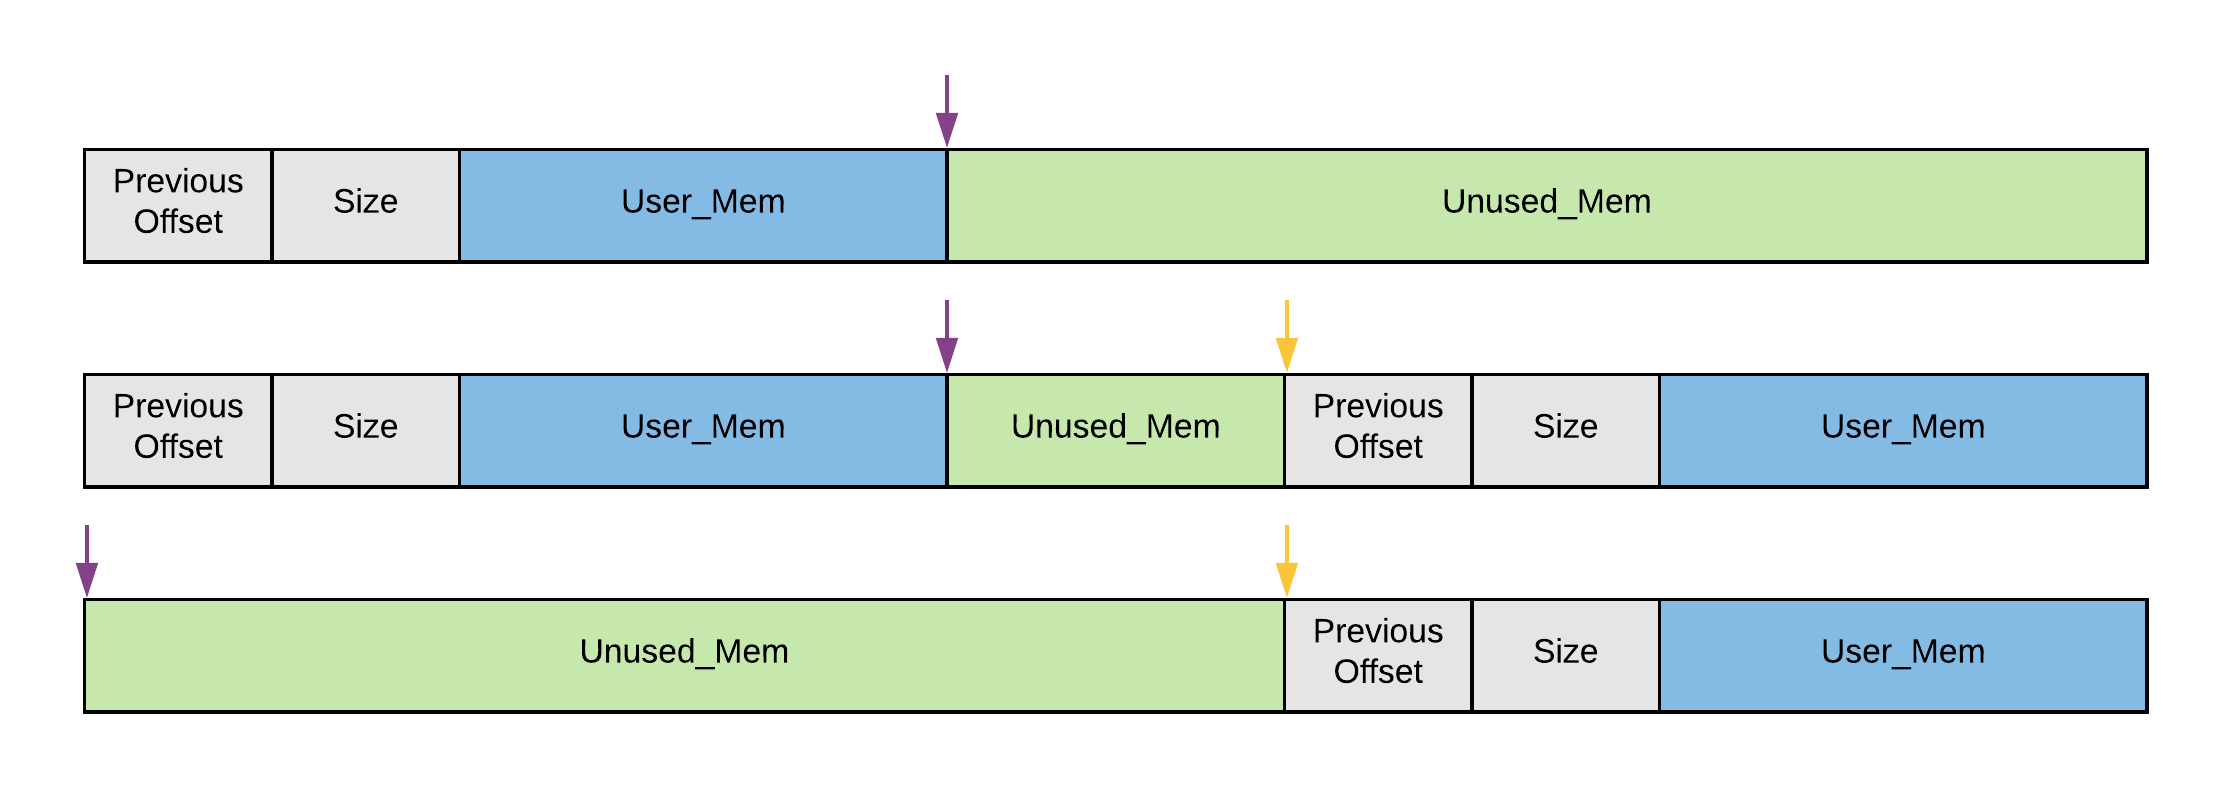
\includegraphics[width=\linewidth]{PICs/double_stack_alloc.png}
	\caption{A double-ended stack-based allocator's internal state. Growing from both sides it needs to be ensured that the internal pointers to not overlap.}
	\label{fig:double_stack_alloc}
\end{figure}

\noindent
When growing from both side, the front pointer advances into the direction of the allocator's end while the back pointer moves to the start. The allocator has to be aware of the possible situation when the two pointer would overlap. This has to be avoided because if one advances the other one, the integrity of issued allocation cannot be ensured. A double-ended stack-allocator is from great benefit when data exists in a compressed and decompressed state. Taking the example of a game world level, the compressed chunk could be loaded by one side, while the decompression allocates memory from the other side.

The last strategy implemented is a \textit{pool allocator}, used for allocation of same-sized elements. Because allocations and deallocations could happen rather frequently when dealing with many small objects, such as particles or other volatile components, they should be fast. A pool allocator allows for allocations and deallocations in a magnitude of O(1). The big-O notation describes the magnitude of O(1) to not scale with the amount of elements stored in a collection. There is one well-known data-structure that satisfy this constraint and that is a linked list. But using a standard list would introduce both, an memory and management overhead because nodes need to allocated and all of them need to be stored somewhere. The technique used in the pool allocator is called an \textit{intrusive linked list} and it comes with no overhead but a single additional pointer. This kind of list lives inside the pooled elements, but only in the ones currently not used. This requires the pooled elements to be at least as large as a \texttt{void*} on the current platform. Listing \ref{lst:freelist_ctor} showcases how such an intrusive linked list is created into a pre-allocated block of memory.\\

\begin{lstlisting}[caption={Constructor of the FreeList class in the C++ project. It showcases how the list is created in a pre-allocated memory region.}, label={lst:freelist_ctor}, language={C++}]
sp::core::FreeList::FreeList(void* memoryBegin, void* memoryEnd, size_t chunkSize)
: m_nextChunk(nullptr)
{
const ptrdiff_t memoryBlockLength = pointerUtil::pseudo_cast<char*>(memoryEnd, 0) - pointerUtil::pseudo_cast<char*>(memoryBegin, 0);
const size_t elementCount = memoryBlockLength / chunkSize;

char* memory = pointerUtil::pseudo_cast<char*>(memoryBegin, 0);
m_nextChunk = pointerUtil::pseudo_cast<FreeList*>(memory, 0);
memory += chunkSize;

FreeList* current = m_nextChunk;
for (size_t i = 0; i < elementCount - 1; ++i)
{
current->m_nextChunk = pointerUtil::pseudo_cast<FreeList*>(memory, 0);
current = current->m_nextChunk;
memory += chunkSize;
}
current->m_nextChunk = nullptr;
}
\end{lstlisting}

\begin{figure}[h!]
	\centering 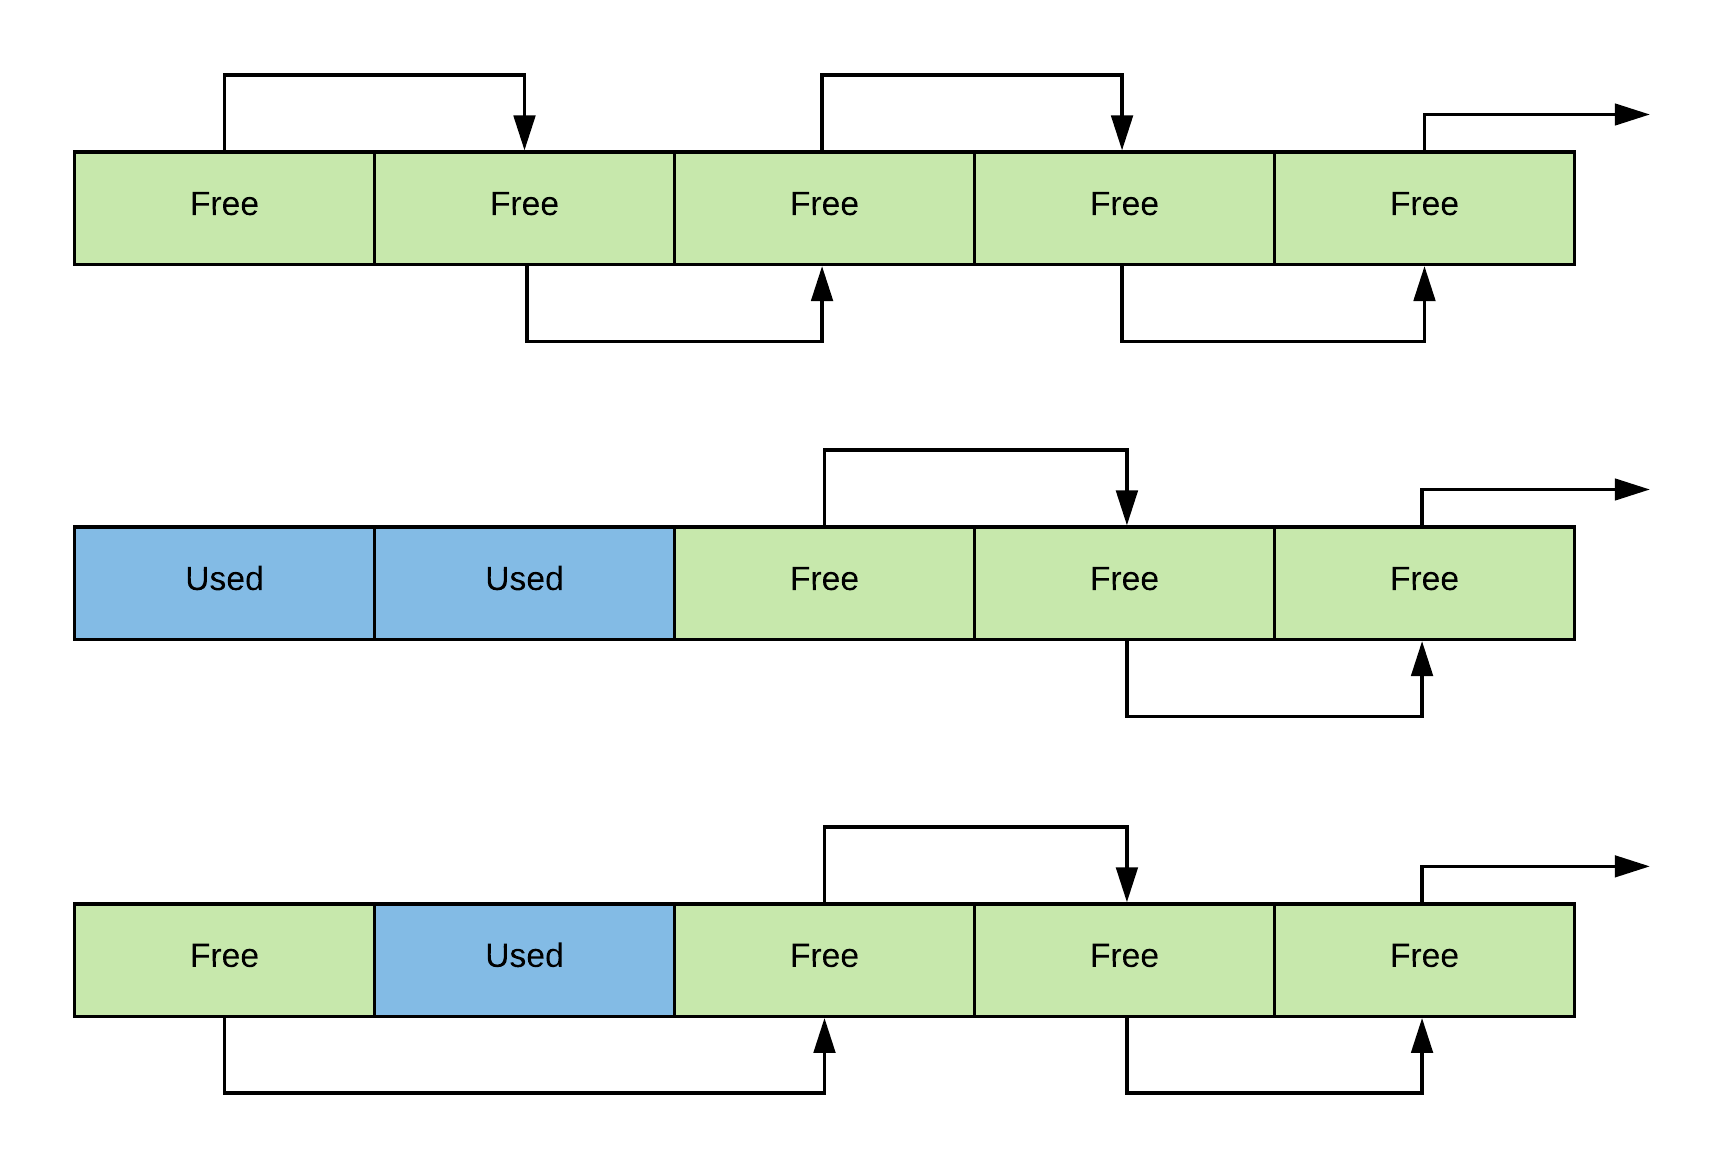
\includegraphics[width=\linewidth]{PICs/pool_alloc.png}
	\caption{A pool allocator including the pointers of the freelist, which allows for O(1) allocation and deallocation of pooled elements.}
	\label{fig:pool_alloc}
\end{figure}

\noindent
\\
With this no overhead data structure in place a user can request an element and deallocate it in O(1). One additional detail is related to how alignment and offset parameters work with the pool allocator. When creating it, the user has to provide the maximum alignment and maximum size of one element. With this information, the allocator computes the minimal chunk size of a single block to fulfill the alignment request. Other than with all previous allocators the offset has to be provided upon construction instead of per allocation. With the minimal chunk size calculated and the offset defined constantly for every element the allocator can fulfill allocation requests with an alignment requirement up to the defined maximum. This can be done because if an element is aligned to N, it is also aligned to all power of twos smaller than N. To explain this with an example, if address A is aligned to 16 bytes, it is also aligned to 8, 4 and two and can therefore serve as the storage location for objects having such alignment requirements. Figure \ref{fig:pool_alloc} shows how the freelist works when an allocation is done and how the pointers are bend when an object is returned.

Additionally to the benefits described above a pool allocator can be enhanced and turned into a growing version. In certain situations it can be useful to have the capability to grow as soon as an allocation request fails because of exhausted memory. The C++ project includes an example implementation of a growing pool allocator that is allowed to grow until it reaches a predefined maximum size constraint. The growing behavior is implemented by using \textit{virtual memory api} provided by the core library.

Although custom allocators can boost an applications performance when used in the right situations, they have limited capabilities for discovering erroneous usage and memory bugs. Because finding such bugs can be hard without any helping utilities the implemented memory feature exposes some debugging capabilities to find common bugs. How they work and which bugs they can warn about is described in the following section.

\subsection{Bounds checker}

To harden an engine's memory system it has to prove some mechanism to prevent or at least detect memory bugs. Some of them that can rather easily be detected are memory leaks and stomps. While a memory leaks describes an allocation that was not deallocated and therefore cannot be used anymore, a stomp corrupts or overwrites memory outside of the allocation's range. The author decided to only implement a capability to detect memory stomps in that thesis due to time constraints. It was decided that more time shall be invested into the different allocators and the other subsystems instead.

A technique that is used for detecting memory stomps is called \textit{bounds checking}. One of the simple variants of it is to insert some markers, also called \textit{canaries}, before and after a user's memory block. When the user frees an allocation again, it is checked whether the inserted canaries still hold the marker values or not. If the either one of the front or end canary was corrupted, an assertion is triggered notifying the programmer that a memory stomp has occurred. There are more advanced approaches that check the integrity of all canaries at every allocation and deallocation made, which allows the for faster error detection for the cost of more computational effort. 

\begin{figure}[h!]
	\centering 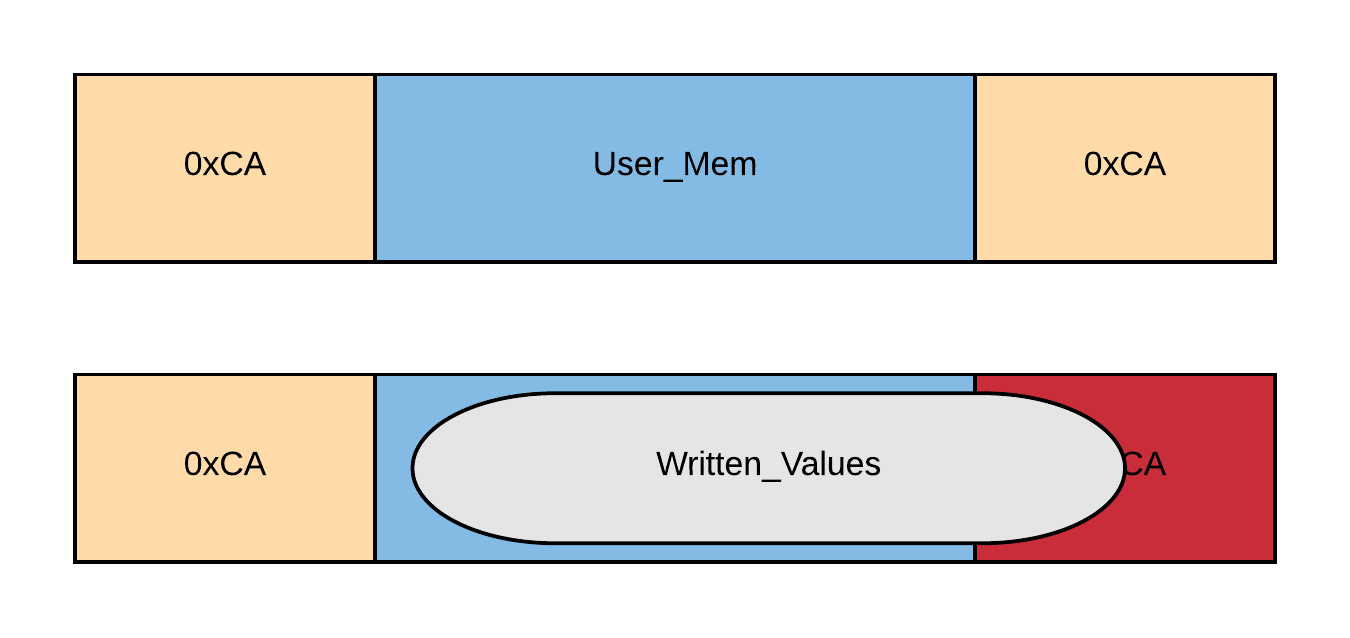
\includegraphics[width=\linewidth]{PICs/canaries.png}
	\caption{Top: an allocation wrapped by valid canaries. Bottom: a value was written into the memory, overflowing its bounds and therefore invalidating the back canary.}
	\label{fig:canaries}
\end{figure}

\noindent
The value chosen for the canaries often is one that is not commonly seen in the patterns of other allocations. In the thesis implementation each canary occupies 4 bytes in memory, being implemented by a 32-bit unsigned integer, and the stored marked value is \texttt{0xCA} in hexadecimal. Such a value is also easily detectable when debugging the application and inspecting the memory. Because using an additional bounds checker that wraps every allocation, the memory system has somehow to ensure that a memory block returned by an allocator is aligned although it also needs to provide extra space for the canaries. That's one of the situation why every allocator can take an additional \textit{offset} parameter. When an offset of X bytes is provided, the allocator ensures that there are exactly X bytes space before the aligned pointer. So if an allocation request with an offset of 4 and an alignment of 16 is issues, the allocator returns a memory block that, if offset by 4 bytes, provides an alignment of 16. Figure \ref{fig:offset_alloc} showcases how an allocation with an offset parameter can look like. Because it would be rather unergonomic to have to do this for every allocation done in the whole engine, the later described memory realm will show how to combine allocators and bounds checking to automate this step.

\clearpage

\begin{figure}[h!]
	\centering 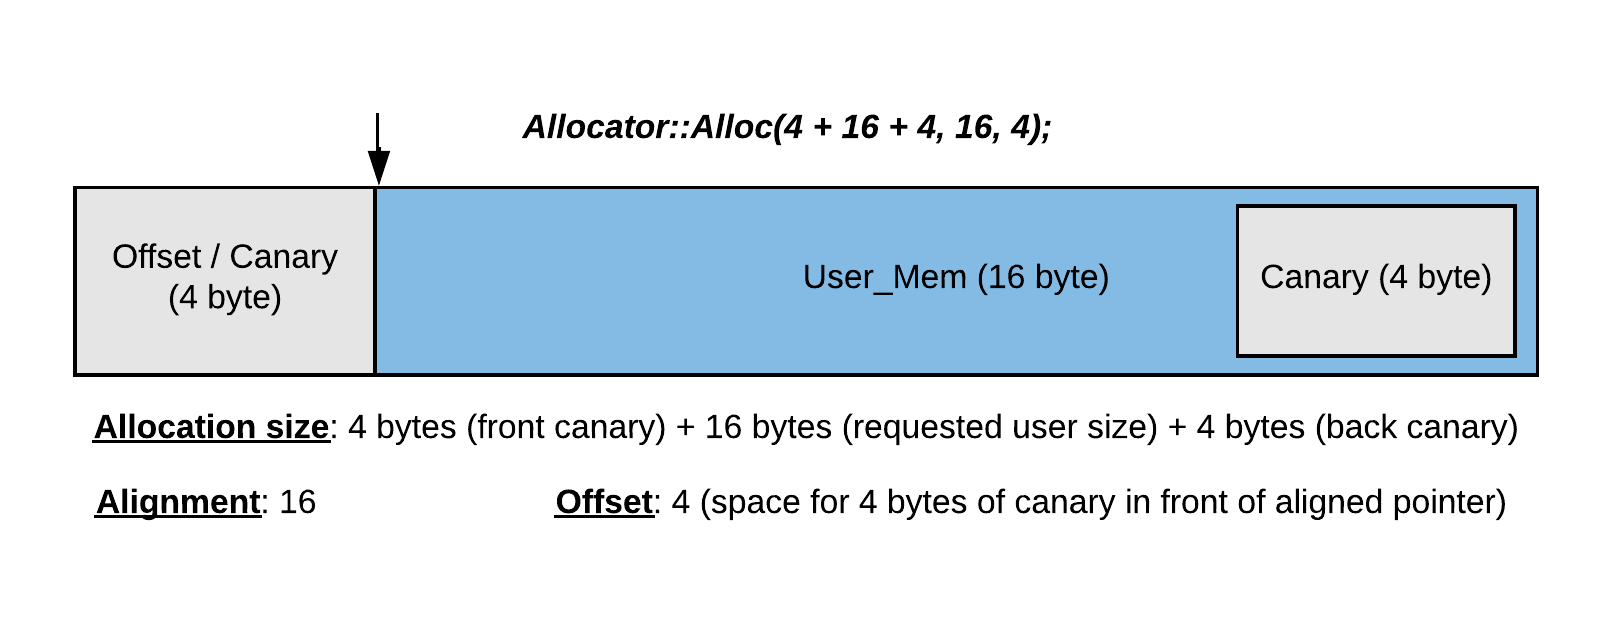
\includegraphics[width=\linewidth]{PICs/offset_alloc.png}
	\caption{Illustrating the structure of a memory block allocated with an offset parameter. To also have space for the second canary, the allocation size if increased by 4 bytes.}
	\label{fig:offset_alloc}
\end{figure}

\noindent
As it can be seen the requested offset bytes are right in front of the aligned pointer that is later handed to the user. Because an additional 4 bytes of space is also needed for the canary at the block's back-end, the allocation size has to be increased by 4 bytes to allow the bounds checker writing to that address. The interface for the bounds checker written in Rust can be seen in Listing \ref{lst:rust_bounds_check}.\\

\begin{lstlisting}[caption={Base trait of every bounds checker in the Rust memory system.}, label={lst:rust_bounds_check}, language={C++}]
pub trait BoundsChecker {
	unsafe fn write_canary(&self, memory: *mut u8);
	fn validate_front_canary(&self, memory: *const u8);
	fn validate_back_canary(&self, memory: *const u8);
	fn get_canary(&self) -> u32;
	fn get_canary_size(&self) -> u32;
}
\end{lstlisting}

\noindent
The same interface is used in the C++ implementation. It has to be mentioned that there are two methods for both canary locations to allow meaningful assert messages when a corrupted value was detected. The next section is going to show a method for combining both every allocation strategy with every implemented bounds checking variant in a flexible and extensible way.

\subsection{Memory realm}

With allocators and bounds checking facilities in place, the memory system needs a way to expose them to a user in an ergonomically way. Although the different parts can already be used without any further abstraction, that way would be rather unergonomic for a programmer to use. In order to expose a more robust and flexible \ac{API}, the memory system contains \textit{memory realms}. This type is an abstraction put on top of allocators and bounds checking to combine them. Both, C++ and Rust, make use of generic code to implement the memory realm. Listing \ref{lst:cpp_mem_realm} shows a partial implementation lacking some details about special member functions. \\

\begin{lstlisting}[caption={Implementation of the memory realm in C++. Some implementation deatils were omitted.)}, label={lst:cpp_mem_realm}, language={C++}]
template <typename Allocator, typename BoundChecker>
class MemoryRealm : public MemoryRealmBase
{
public:
	explicit MemoryRealm(size_t bytes)
	: m_allocator(bytes)
	{}
	
	template<typename MemoryProvider>
	explicit MemoryRealm(MemoryProvider& memoryProvider)
	: m_allocator(memoryProvider.start(), memoryProvider.end())
	{}
	
	void* Alloc(size_t bytes, size_t alignment) override
	{
		const size_t totalMemory = m_boundsChecker.CANARY_SIZE + bytes + m_boundsChecker.CANARY_SIZE;
		
		char* memory = static_cast<char*>(m_allocator.Alloc(totalMemory, alignment, m_boundsChecker.CANARY_SIZE));
		
		m_boundsChecker.WriteCanary(memory);
		m_boundsChecker.WriteCanary(memory + m_boundsChecker.CANARY_SIZE + bytes);
		
		return memory + m_boundsChecker.CANARY_SIZE;
	}
	
	void Dealloc(void* memory) override
	{
		char* allocatorMemory = static_cast<char*>(memory) - m_boundsChecker.CANARY_SIZE;
		
		m_boundsChecker.ValidateFrontCanary(allocatorMemory);
		const uint32_t allocationSize = static_cast<uint32_t>(m_allocator.GetAllocationSize(allocatorMemory));
		m_boundsChecker.ValidateBackCanary(allocatorMemory + m_boundsChecker.CANARY_SIZE + allocationSize);
		
		m_allocator.Dealloc(allocatorMemory);
	}
	
	void Reset(void) override
	{
		m_allocator.Reset();
	}
	
	~MemoryRealm() = default;

private:
	Allocator m_allocator;
	BoundChecker m_boundsChecker;
};
\end{lstlisting}

\noindent
The code sample shows that a realm takes two template parameters defining the allocator and bounds checker used. An advantage of this design, also being named \textit{policy-based design}, is that each realm can be rather easily configured to use every allocator and every bounds checker, if they adhere to the same interface. To give an example, one memory realm could use a linear allocator with canary-based bounds checking during development and is exchanged by a realm using the same linear allocator but with a bounds checker that only has no-op methods. The bounds checker used in release implemented each of its methods empty, allowing the called functions to yield a no-op when being compiled for release or retail mode. With this approach a user can define memory arenas in a flexible way, creating the ones fitting a certain use case. This approach could even be enhanced, as Stefan Reinalter also describes in his blog \cite{MOL_MS_5}, by adding facilities for handling multi-threaded access and memory tracking. These parts can then also be added as template parameters and increase the possibilities a programmer has.

While the C++ implementation uses templates, the Rust approach is based upon the feature of \textit{generics}. Combined with traits the Rust implementation allows for also constraining the passed types and force them to implement a certain interface. Although that functionality would also be implementable in C++, Rust includes it in its core language, while the C++ mechanism would be a custom creation (\textit{type traits} or \textit{concepts}). In Listing \ref{lst:rust_trait_bound_basic} \& \ref{lst:rust_trait_bound_typed} it can be seen Rust's trait bounds can be useful when implementing a generic abstraction where an used type has to provide certain functionality defined by an interface.\\

\begin{lstlisting}[caption={Rust interface of the basic memory realm allowing only basic allocators.}, label={lst:rust_trait_bound_basic}, language={C++}]
pub struct BasicMemoryRealm<A: Allocator + BasicAllocator, B: BoundsChecker + Default> {
	allocator: A,
	bounds_checker: B,
}
\end{lstlisting}

\begin{lstlisting}[caption={Rust interface of the typed memory realm.}, label={lst:rust_trait_bound_typed}, language={C++}]
pub struct TypedMemoryRealm<A: Allocator + TypedAllocator, B: BoundsChecker + Default> {
allocator: A,
bounds_checker: B,
}
\end{lstlisting}

\subsection{Idiomatic Rust implementation}

While the C++ implementation returns raw pointers and indicates error states with a \texttt{nullptr}, the Rust project features a safe wrapper around allocations to also showcase an approach using idiomatic Rust principles. To allow the system to be used in safe Rust, the author needed a way to somehow make the allocation \ac{API} more robust and safe. To reach this goal, the \texttt{Box} type of the standard library served as a reference. A \texttt{Box} is a way to heap allocate in Rust and it follows the \ac{RAII} idiom as many other Rust implementations. Because the current version of the language does not feature custom allocators in a stable way, the author implement a custom type calls \texttt{AllocatorBox}. It was responsible for managing the allocated memory block and to free it properly when it is dropped. To do so it needed to hold a reference to the allocator the memory block comes from the the block itself. This also ensures, that an allocation can not live longer than the allocator it came from due to Rust's lifetime rules and the borrow checker.\\

\begin{lstlisting}[caption={AllocatorBox abstraction to allow \ac{RAII} management of allocations.}, label={lst:rust_allocator_box}, language={C++}]
pub struct AllocatorBox<'a, T: 'a + ?Sized, A: 'a + Allocator + ?Sized> {
	instance: Unique<T>,
	allocator: &'a A,
}

// ...

impl<'a, T: ?Sized, A: Allocator + ?Sized> Drop for AllocatorBox<'a, T, A> {
fn drop(&mut self) {
	unsafe {
		intrinsics::drop_in_place(self.instance.as_ptr());
		self.allocator.dealloc_raw(MemoryBlock::new(self.instance.as_ptr() as *mut u8));
	}
}

\end{lstlisting}

\noindent
Listing \ref{lst:rust_allocator_box} showcases the members of an \texttt{AllocatorBox}. It uses the \texttt{Unique} type to indicate that it is the only owner over the value and a reference to the allocator the memory block came from. At the bottom it can be seen how the \texttt{Drop} trait is implemented and what happens when an \texttt{AllocatorBox} goes out of scope. The owned instance is dropped and then a memory block is created from the owned pointer. That block is handed back to the allocator it came from, properly releasing memory as soon as it is not needed anymore. 

\newpage

\section{Containers} \label{container_impl}

With the memory system as a quite low-level one, the second part of the implementation section focuses on a slightly more high-level library featuring three different kind of containers. A container serves the purpose of holding several elements, allowing to add and access them. The author decided to implement the following three collections, all of them capable of being used at runtime or for implementing tools.

\begin{labeling}{handle map}
	\item [vector] dynamically size array, storing elements in a contiguous memory block
	\item [handle map] collection that internally stores items contiguous in memory 
	while external handles to them will be kept intact
	\item [ringbuffer] collection allowing for reading and writing to it
	with the capability of wrapping around at the end
\end{labeling}

The following sections will each describe how the collection works and how it was implemented in C++ and Rust.

\subsection{Vector}

A vector is a collection most typically found in the standard library of most programming languages. With \texttt{std::vector<T>} and \texttt{Vec<T>}, both C++ and Rust, already provide an implementation to be used by a programmer. This collection can also be described as an array that is able to grow on demand. So while it is preferable to use fixed-size arrays due to reasons such as memory waste, book-keeping overhead and performance, there are some situations where the required size of an array cannot be known at compile-time. That are the situations where a vector is the tool of choice. But why is there the need for implementing such a collection if the languages already provide one? The reason is, as often in the world of game engines, performance. Standard library collections fulfill the need of being portable and that's the reason why there are several ways how the performance of them can be improved when certain unknowns are replaced by the knowledge of a machine's capabilities and usage patterns. 

The difference between standard library implementations and the one chosen by the author is the way the collection retrieves its memory and how the growth is handled. Vectors commonly use the languages default memory allocation system to allocate space for its elements. While normally this is not a problem, it can become one as soon as the vector's current capacity is exhausted. During this situation, the vector allocates a new space that is bigger than the current one, moves all elements into that space and frees the old one. This can be either done by using allocation capabilities such as \texttt{realloc}, provided by the default allocator, or manually. Both of these approaches can lead to the problem that for a short time, the old and the new memory block are allocated at the same time, wasting memory until the old one is freed. The chosen implementation aims to avoid this problem by using the virtual memory system of the \ac{OS} to allocate and free space.

\subsubsection{Spark Vector}

Contrary to the standard libraries vectors, the one implemented for Spark only allocates its memory via the virtual memory system of the \ac{OS}. When a new one is created, it reserves virtual address space up to one \ac{GB}. Due to that fact the implementation is only useful on 64-bit platforms to the bigger address space available on them. Whenever elements are added, or pushed, to the vector, a check is performed whether it needs to grow or not. If the check results that growing the collection is necessary, physical pages meeting the required capacity are committed. And here lies the different to the standard vector implementation. While normally in this situation memory usage could nearly be doubled, Spark's vector does not need to allocate or reallocate a new block. Because all of the already reserved virtual address space lies contiguous in memory, relocation of the previously owned elements is not needed and the new elements are just appended at the end of the already committed pages.\\

\begin{figure}[h!]
	\centering 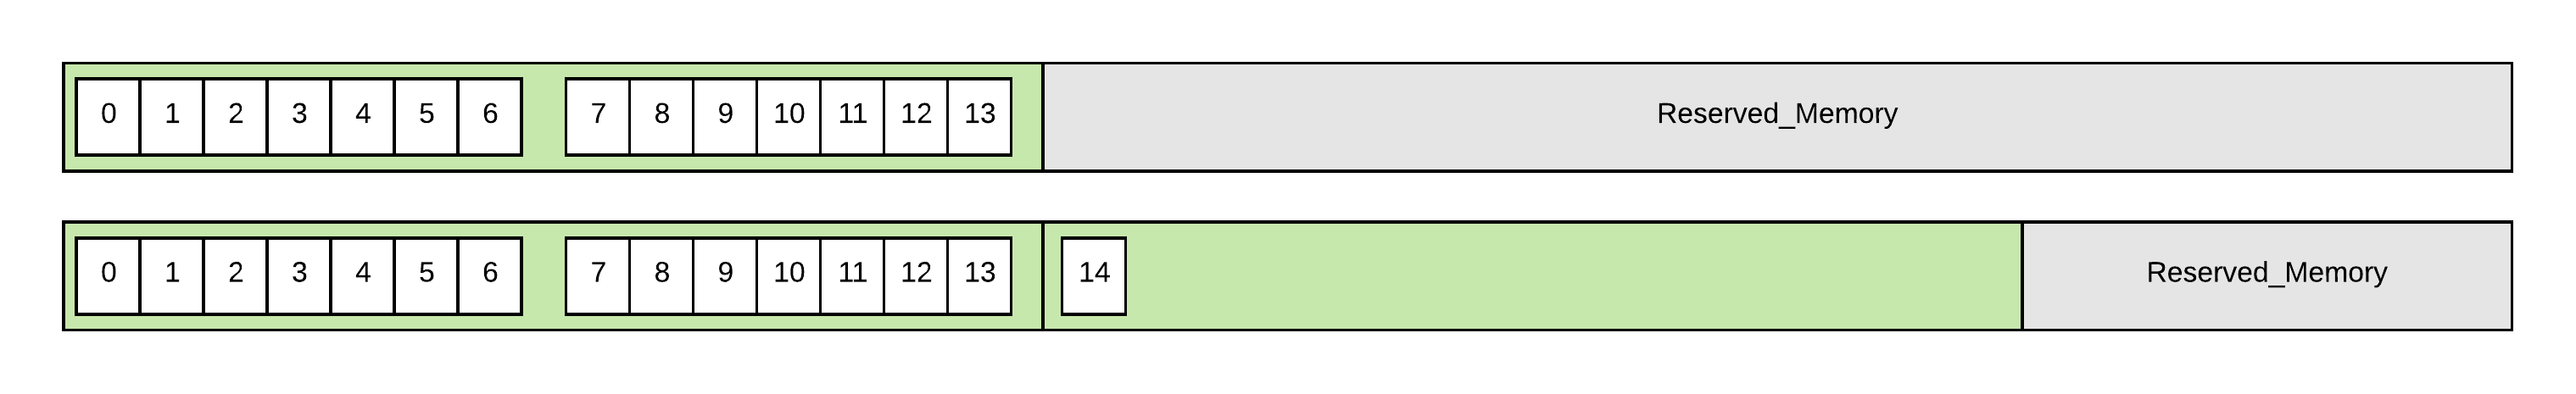
\includegraphics[width=\linewidth]{PICs/vector_growth.png}
	\caption{Illustrating the growing process of Spark's vector.}
	\label{fig:vector_growth}
\end{figure}

\noindent
A visual description of the vector growth can be seen in Listing \ref{fig:vector_growth}. The figure shows the situation where a new element is added to an already exhausted vector. To fit the element into the collection, another range of memory pages is committed. The amount of the newly allocated capacity is determined by fixed growing rules, ranging from twice the current size to more exotic growth patterns. What exactly is done during the growing process of the vector can be seen in Listing \ref{lst:vector_growth}. This code sample shows how the \texttt{grow} method is implemented in Rust. The C++ function is now shown because they logically work in the same way only differing in syntax.\\

\begin{lstlisting}[caption={Growth function of the Spark vector in Rust.}, label={lst:vector_growth}, language={C++}]
fn grow(&mut self, bytes: usize) {
	{
		let virtual_address_space_exhausted = self.internal_array_begin.as_ptr() as *mut u8 == self.virtual_mem_end;
		debug_assert!(!virtual_address_space_exhausted, "Not enough address space to grow further");
	}
	
	let page_bytes_to_grow = math_util::round_to_next_multiple(bytes, virtual_mem::get_page_size());
	
	let is_enough_space_for_requested_pages = unsafe { self.internal_array_end.offset(page_bytes_to_grow as isize) <= self.virtual_mem_end };
	let grow_by_bytes = if is_enough_space_for_requested_pages {
		page_bytes_to_grow
	}
	else {
		let remaining_virtual_address_space = self.virtual_mem_end as usize - self.internal_array_end as usize;
		math_util::round_to_previous_multiple(remaining_virtual_address_space, virtual_mem::get_page_size())
	};
	
	let ptr = match { virtual_mem::commit_physical_memory(self.internal_array_end, grow_by_bytes) } {
		None => ptr::null_mut(),
		Some(mem) => mem,
	};
	
	if ptr.is_null() {
		debug_assert!(true, "Vector run out of memory due to an unknow error");
	}
	
	self.internal_array_end = unsafe { ptr.offset(grow_by_bytes as isize) };
	self.capacity = self.capacity + (grow_by_bytes / mem::size_of::<T>());
}
\end{lstlisting}

\noindent
While growing a vector is normally straight forward, there is a an edge case if the demanded capacity is not covered by available address space. If this situation occurs the vector does not assert or fail, but allocates all available pages until the end. That is the only case where the defined growing rule is ignore to utilize the available memory limits till the maximum. At the end, if committing the physical pages succeeded, the internal state, including current array end and capacity, is updated. It has to be mentioned that due to the virtual memory system, the vector can only grow in a multiple of the \ac{OS}'s page size.

\subsection{Handle Map}
\blindtext
\subsection{Ringbuffer}
\blindtext

\section{Entity Component System} \label{ecs_impl}
\blindtext
\subsection{SPECS}
\blindtext
\subsection{Entities \& Components}
\blindtext
\subsection{World}
\blindtext
\subsection{Systems}
\blindtext